\chapter{Protocole expérimental}
	\section{Dispositif}
	\subsection{Hypothèses de travail}
	\par qsd	
	
	\subsection{Tache à effectuer}	
	\par petite cible à viser, appuyer sur une manette, pas de questionnaires mais quelques renseignements (âge, vision, gamer), (fig. flowchart 2)
	
	\par différentes luminances (ordre aléatoire) et différents contrastes (re ordre aléatoire), 1h de warmup selon recommendations de la CIE (IEC 61966-6:2005)
	
	\subsection{Sujets \& matériel}
	\par On réunit un total de 32 sujets (Fig. \ref{fig:expe_sujets}) pour cette expérimentation, les même que pour l'étude expérimentale décrite dans la partie précédente (Cf.  \ref{chap:sdr_etude_experimentale}). Ces derniers sont volontairement choisis jeunes (entre 20 et 27 ans) pour minimiser l'impact de la dégradation de la vision avec l'âge. Tous les sujets ont donc une vision parfaite, ou corrigée et assimilée parfaite. La moyenne d'âge est de 25 ans, avec un écart-type de 1,8 ans.
	
	\par De même, les conditions matérielles sont identiques que pour la première expérimentation: dans un simulateur de type CAVE (Cf. \ref{tab:cave_dimensions} pour les dimensions), les sujets sont assis dans un fauteuil de voiture, la tête bien calée dans l'appui-tête. Néanmoins, pour cette expérimentation, les sujets n'utilisent pas de lunettes stéréoscopiques. L'expérimentation se fait donc en affichage monoscopique. Les sujets sont placés de manière à avoir les yeux à 2 mètres du centre de l'écran <<~principal~>>, la face avant.
	
	\begin{figure}
		\centering
		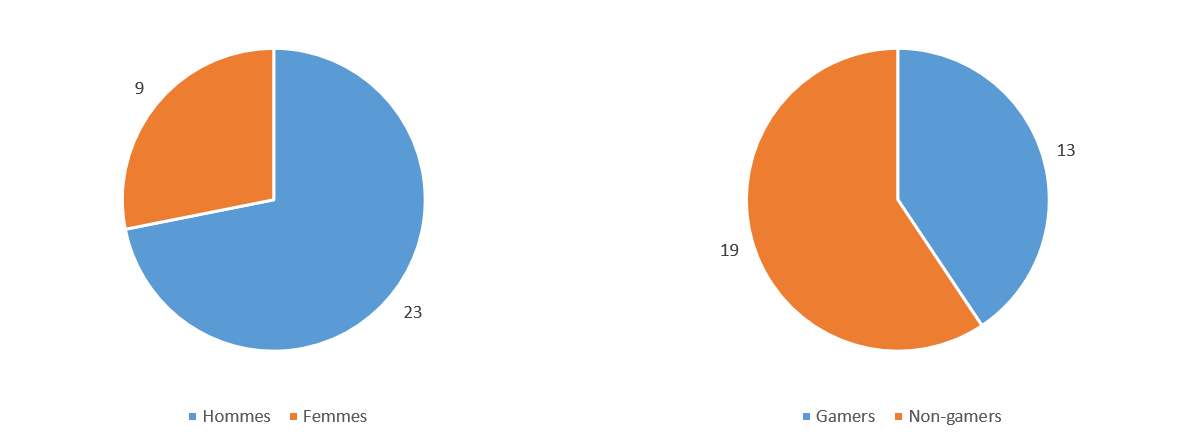
\includegraphics[scale=0.8]{Figures/SubjectsCharts}
		\caption{Répartitions des sujets pour les expérimentation de contraste/luminance et de comparaison objective/subjective.}
		\label{fig:expe_sujets}
	\end{figure}
	
	\section{Choix des conditions expérimentales}
	\subsection{Luminance}
	\par qsd
	
	\par certaines conditions sortent du champ du modèle (les plus basses luminances): permet d'extrapoler les résultats en cas de fonctionnement des plus hautes luminances
	
	\subsection{Contraste}
	\par qsd
	
	\par Tous les contrastes sont proposés au sujet et dans un ordre aléatoirement mélangé grâce à l'algorithme suivant
	
	% block quote algo en pseudo code
	
	
	
\chapter{Résultats}
	\section{Prédictions du modèle théorique}
	\par qsd
	
	\section{Mesures réelles}
	\par qsd